% Shared preamble for the English summaries in this repository.
\documentclass[11pt,a4paper]{article}
\usepackage[margin=2.2cm]{geometry}
\usepackage[T1]{fontenc}
\usepackage[utf8]{inputenc}
\usepackage{lmodern}
\usepackage{amsmath,amssymb}
\usepackage{graphicx}
\usepackage{booktabs}
\usepackage{enumitem}
\usepackage[hidelinks]{hyperref}
\setlist{itemsep=2pt,topsep=4pt}
\setlength{\parindent}{0pt}
\setlength{\parskip}{5pt}
\graphicspath{{figures/}}
\newcommand{\summaryheader}[3]{%
  \begin{center}
    {\Large\bfseries #2}\\[3pt]
    {\large #1}\\[3pt]
    {\small Arshia Goshtasbi \textbullet{} MSc Electrical Engineering (Control), Iran University of Science and Technology \textbullet{} #3}
  \end{center}
  \vspace{2pt}\hrule\vspace{8pt}
  \noindent\textit{English summary of my original Persian report, which is kept as a PDF in this folder.}\par}

\begin{document}
\summaryheader{Adaptive Control, Homework 2}{Recursive Least Squares, Excitation and Forgetting (Åström \& Wittenmark, Simulations 2.12--2.16)}{Autumn 1404 (2025)}

All models are subsystems of \texttt{Q2\_All.slx}. In each one an RLS estimator identifies the parameters of a discrete-time plant, and I compared my plots with the book's.

\begin{description}
  \item[Simulation 2.12 (persistent excitation).] Three inputs were compared: the book's first input, a square wave, and an input from the class example. The first and third have little persistence of excitation, so they are not suitable for identification. The square wave excites the plant better, and the simulation showed this, as in the book.
  \item[Simulation 2.13.] The book's two cases (a) and (b), reproduced.
  \item[Simulation 2.14 (forgetting factor).] RLS with $\lambda=1$, $0.999$, $0.99$ and $0.95$, for two input cases.
  \item[Simulation 2.15.] As $\lambda$ decreases, the estimates fluctuate more, because the estimator effectively bases its estimates on fewer past samples.
\end{description}

\begin{center}
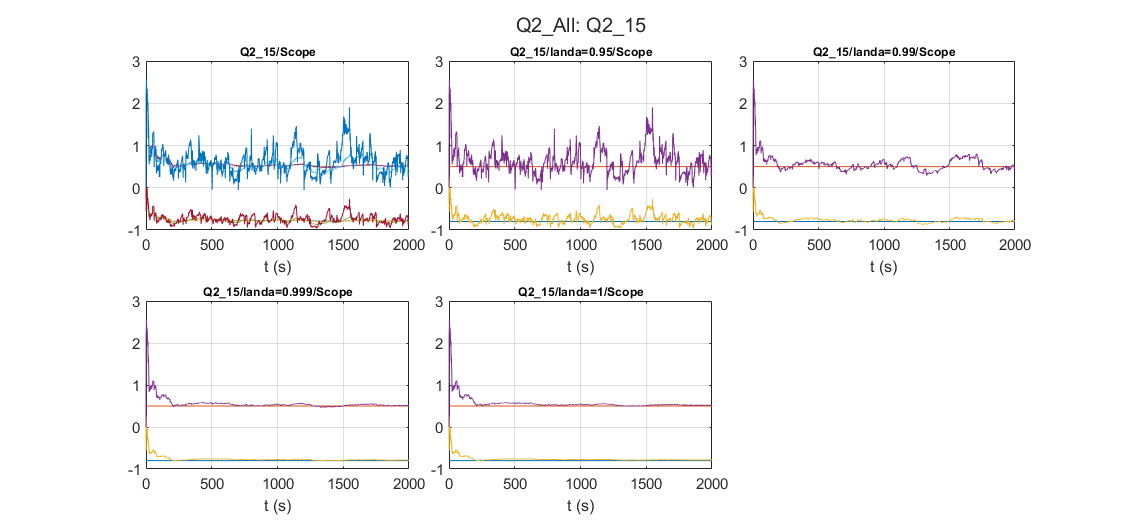
\includegraphics[width=0.9\linewidth]{Q2_15.png}\\[2pt]
{\small Re-run in R2023b: simulation 2.15, estimates for different forgetting factors.}
\end{center}
\end{document}
